\chapter{Background}
%Starting my final year project at the Electronic Vision(s) group, I soon realized the diversity of their research. 
From the biological view of the human brain to electronic circuit laws further to machine learning algorithms, the required knowledge to work in the field of neuromorphic computing is broad and manifold. In the next sections, I will introduce the most important concepts and physical backgrounds upon which the presented research in this works is based on. Starting with the biological background of neurons and an overview of deep learning with \glspl{ann}, the transition to \glspl{snn} and their coding schemes will be made.

\section{The Biological Neuron}

It is estimated that the human brain contains around $10^{11}$ neurons (\cite{numberofneurons}). Neurons come in different shapes, sizes and functions. However, as depicted in \cref{biossynapse} in most cases they can be divided into three separate functional parts: dendrites, soma and axon (c.f. \cite{gerstner2014dynamics}). The dendrites gather all inputs from various sources and forward them to the soma where the received information is processed. In particular, the soma integrates the input and once exceeding a threshold it will initiated a response, which is then relayed by the axon to other neurons. This response has the shape of a short chemical pulse (spike) or a cascade of such spikes (burst). Depending on the nature of neuron the response can either excite or inhibit the receiving neuron's membrane (soll hier eine citation zu dales law?) and thus lead to an in- or decrease of its membrane potential. A \emph{synapse} connects two neurons. Usually a neuron hast up to $10^4$ \emph{postsynaptic} partners. This terminology is derived from an actual physical gap at the synapse - the synaptic cleft. The \emph{presynaptic} neuron then releases various neurotransmitter to overcome the cleft and once a transmitter has docked to a corresponding receptor on the other side, the activation of ion channels convert the chemical transmission back into an electrical signal.\\

\begin{figure}
	\begin{subfigure}{0.5\textwidth}
		\centering
		\caption{}
		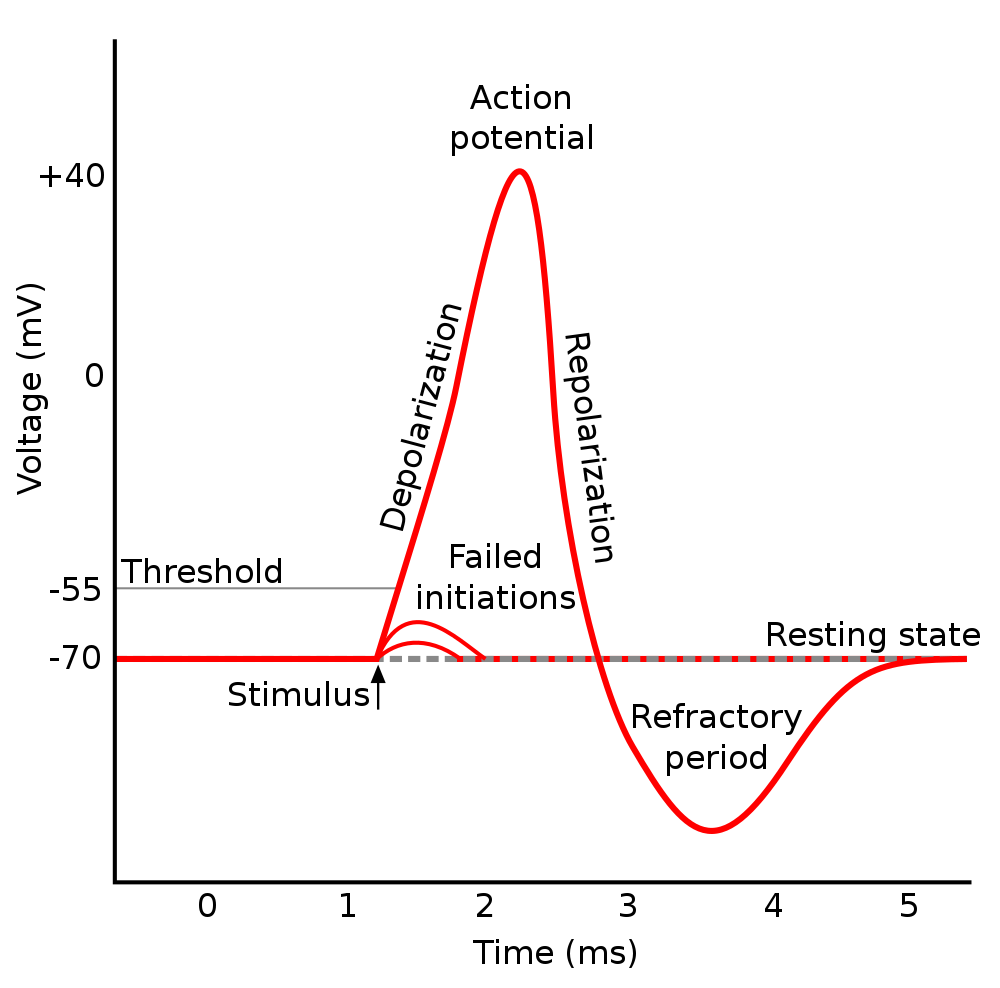
\includegraphics[width=0.8\linewidth, valign=t]{figures/action_potential.png}
		\label{actionpotential}
	\end{subfigure}
	\begin{subfigure}{0.5\textwidth}
		\centering
		\caption{}
		\vspace{0.5cm}
		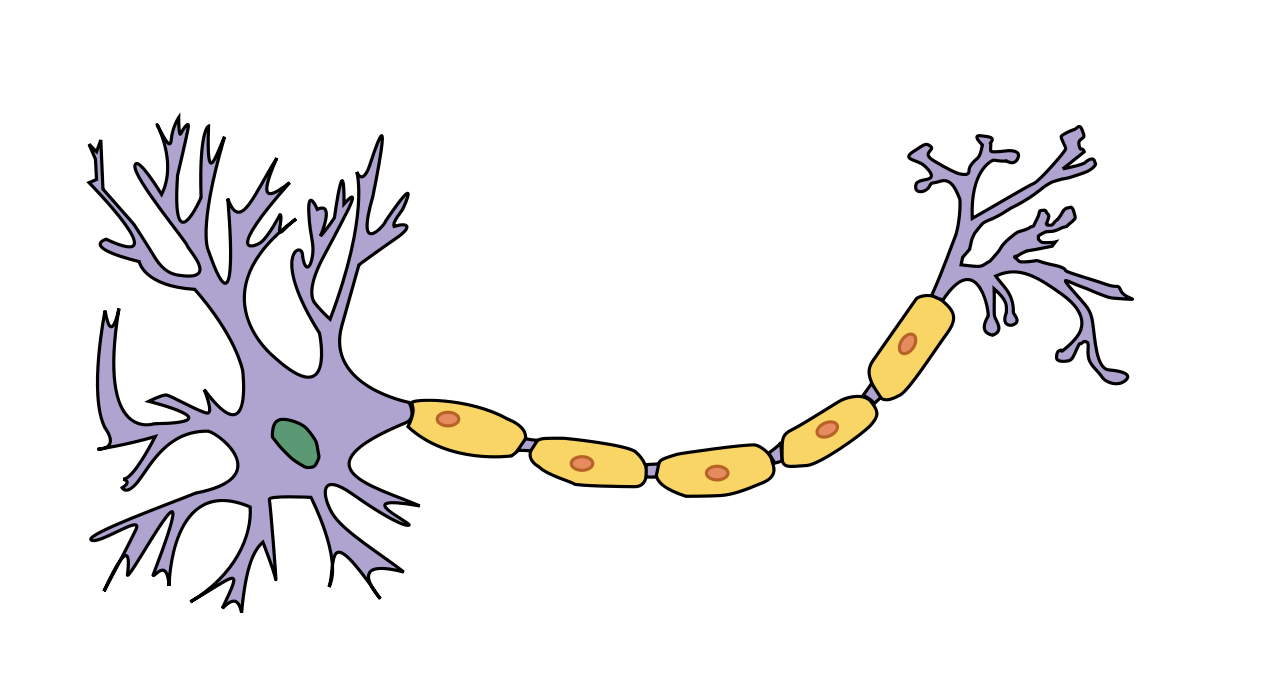
\includegraphics[width=\linewidth, valign=t]{figures/neuron_model.png}
		\vspace{1.5cm}	
		\label{biosynapse}
	\end{subfigure}
	\caption{(\subref{actionpotential}): The response of neuron after exceeding the threshold is called action potential. After a phase of depolarization, the membrane repolarizes and enters the refractory state. (\subref{biosynapse}): Schematics of a biological neuron split into dendrites, soma and axon}
	\label{biologicalneuron}

\end{figure}

The unbalanced ion concentration in and outside of the membrane is restored by ion pumps over time. The equilibrated state of the membrane potential is referred to as the \emph{resting potential}. Once a spike has been fired, the neuron's membrane becomes hyperpolarized and decrease even below the resting potential. At this point it is impossible for the neuron to spike again. The neuron is in a so called \emph{refractory state}. Due to the ongoing hyperpolarization it remains hard but not impossible to fire. The typical dynamics of a membrane potential are depicted in \cref{actionpotential}.





A wide-spread assumption in field of neuroscience is that the exact shape of a spike doesn't carry any relevant information and therefore all spikes can be modeled by a stereotypical shape. The communication between neurons is then encoded in the frequency (\emph{rate coding}) or timing (\emph{time coding}) of exciting and inhibitory spikes. A more detailed description of neural coding schemes is presented in section \ref{deeplearning}. However, recent research (\cite{debanne2013mechanisms}) has suggested that the variate of the shape contains vital information.

\section{Deep Learning}
\label{deeplearning}
Among the many tools machine learning has provided to the scientific community, deep learning is one of the most useful and powerful tool when it comes to solving complex tasks. One approach is to understand such a task in terms of a hierarchy of concepts. Each concept is based upon a combination of simpler ones. Going done on a hypothetical ladder towards the easiest concept available, creates a deep structure with many layers. This is why it's called \textit{deep learning} (\cite{Goodfellow-et-al-2016}).

A popular example of deep learning is a feedforward neural network or \gls{mlp}. In a feedforward network the information is passed from one layer to another. At each layer the input $\mathbf{x}$ is mapped to an output $\mathbf{y} = f(\mathbf{x, \theta})$ by a transferfunction $f$ and a set of parameters $\mathbf{\theta}$. The parameters are then trained in order to obtain the optimal result. The layer structure of such a network is inspired by biological neural networks which is why it is often referred to as \glsfirst{ann}.\\

%Given the task to identify a picture of cat, any computer will have a hard time to map the essential information of the camera's sensor data to the class \textit{cat}. An \gls{ann} solves the problem by learning how to describe the raw data in terms of simpler representations and essentially by combining these simpler representations into a meaningful solution in the last layer - the output layer. The first layer is called input layer and all other layers in between are named hidden layers, since they are usually not visible from the outside.\\


\subsection{Training Methods for \glspl{ann}}
\label{trainingANN}

The learning process of a neural network can be divided into a \emph{forward} and \emph{backward} pass. 

\subsubsection{Forward Pass}
During the forward pass the output value of each node in the network is evaluated. The activation $\mathbf{a}$ of a layer $l$ is given by the product of the input $\mathbf{x}$ with a weight matrix $W^{(l)}$ plus a bias $\mathbf{b}$.
\begin{align}
\label{activation}
\mathbf{a} = W^{(l)} \, \mathbf{x} + \mathbf{b} \left(+ \text{noise}\right)
\end{align}
Depending on the task to the bias and an additional noise term can be vital. The bias allows the network to shift the dynamic range of a single neuron and for certain tasks and network structure \glspl{ann} may perform poorly without the injection of artificial noise.

The output value $\mathbf{y}$ of the layer given by a transfer function $\phi$
\begin{equation}
\label{transferANN}
\mathbf{y} = \phi(\mathbf{a}).
\end{equation}

The choice of the transfer function is to a certain degree free. A \gls{relu}, a hyperbolic tangent ($\tanh$) or a sigmoid are among the most popular ones (see \cref{deeplearning_activation_functions}. However, it is important that chosen function has a non-linear nature, as its gradient won't be able to separate magnitude or sign of the input otherwise. The dependency on the input of the gradient is a vital function for the learning process. 

\begin{figure}
	\begin{subfigure}[c]{0.5\textwidth}
		\centering
		\caption{}
		\inputpgf{figures}{deeplearning_activation_functions.pgf}
		\label{dltransfer}
	\end{subfigure}
	\begin{subfigure}[c]{0.5\textwidth}
		\centering
		\caption{}
		\inputpgf{figures}{deeplearning_activation_functions_derivative.pgf}	
		\label{dltransfergradient}
	\end{subfigure}
	\caption{(\subref{dltransfer}): Some of the most popular shapes for the transfer function are a \gls{relu}, $\tanh$ or sigmoid. (\ref{dltransfergradient}): Training with a linear function would not work, because the gradient is a constant and doesn't discriminate between different inputs. A non-linear transfer function is thus vital to the training. The \gls{relu} is, despite appearing to be a linear function, non-linear}
	\label{deeplearning_activation_functions}
	
\end{figure}

The same principle is applied to all other layers in a forward direction, i.e. the result of the previous layer is the input for the current layer. The weight matrix $W^{\text{(l)}}$ connecting layer $l$ with $l-1$ has the appropriate shape to fit the number of input nodes $n^{\text{(l-1)}}_\text{nodes}$ and the number of nodes in the current layer $n^{\text{(l)}}_\text{nodes}$. (maybe figure with a layer structure, like in mfp talk)

\subsubsection{Backward Pass}
\label{backwardpassANN}
The backward pass computes how the networks parameters $\mathbf{\theta}$ need to be changed to obtain the best result. One approach, called \emph{gradient descent}, minimize a given loss function $\mathcal{L}(\mathbf{\theta})$ by moving along the negative gradient of the $\loss$ , c.f. \cite{Goodfellow-et-al-2016}. The new set of parameters $\mathbf{\theta'}$ is then given by
\begin{equation}
\mathbf{\theta'} = \mathbf{\theta} - \eta \, \nabla\loss(\mathbf{\theta}).
\end{equation}
whereby $\eta$, the learning rate, defines how fast an update is applied. As an example the update of the weight matrices $\delta W^{(l)}$ is computed. The update of bias can be done in analogy to the weights. 

In combination with a cross-entropy loss the choice of a sigmoid transfer function becomes convenient when deriving the parameter changes. First it necessary to know what the loss function looks like. This is why the computation starts from the end of the layer structure, the output layer. The derivative of the sigmoid yields $\frac{\partial \mathbf{y}}{\partial \mathbf{a}} = \frac{\partial \phi(\mathbf{a})}{\partial \mathbf{a}} = \phi (1 - \phi)$ and the derivative of the imposed a cross-entropy loss is given by
\begin{align}
\frac{\partial\mathcal{L}}{\partial \mathbf{y}} = 
- \frac{\hat{\mathbf{y}}}{\mathbf{y}} + 
\frac{1 - \hat{\mathbf{y}}}{1 - \mathbf{y}}
\end{align}
with $\mathbf{y}$ the output and $\hat{\mathbf{y}}$ the target output. The error $\mathbf{e} = \hat{\mathbf{y}} - \mathbf{y}$ can then be rewritten in terms of the partial gradients
\begin{equation}
\Rightarrow \quad \frac{\partial\mathcal{L}}{\partial \mathbf{a}} =
\frac{\partial\mathcal{L}}{\partial \mathbf{y}} 
\; \frac{\partial \mathbf{y}}{\partial \mathbf{a}} =
\hat{\mathbf{y}} - \mathbf{y} = \mathbf{e}.
\end{equation}
Now the weight update $\delta W^{\text{(o)}}$ for the output layer yields 
\begin{align}
\delta W^{\text{(o)}} =& - \eta \frac{\partial \mathcal{L}}{\partial W} 
= - \eta \;
\frac{\partial\mathcal{L}}{\partial \mathbf{y}} \;
\frac{\partial \mathbf{a}}{\partial W}
= - \eta \, (\mathbf{e} \cdot \mathbf{x}^T),
\end{align}
with $\mathbf{x}$ being the input of the output layer, thus the output of the hidden layer.

The result for the hidden layer computes similarly. Again we look at the gradient of the loss function and find
\begin{align}
\frac{\partial\mathcal{L}}{\partial \mathbf{a}} &= \left(W^{\text{(o)}T} \cdot \mathbf{e}\right) \;
\frac{\partial \mathbf{y} }{\partial \mathbf{a}}\\
\Rightarrow \quad \delta W^{\text{(h)}} &= - \eta \;
\left(W^{\text{(o)}T} \cdot \mathbf{e}\right) \;
\frac{\partial \mathbf{y} }{\partial \mathbf{a}} \;
\mathbf{x}^T,
\end{align}
Where $W^{\text{(o)}T}$ denotes the transpose of the weights of the output layer, i.e. the weights connecting the output layer to the hidden layer in backward direction. The backward propagation of the error is name giving and thus it is often referred to as \textit{back propagation}. Despite the great performance for many deep learning tasks, the biological plausibility of propagating the error signal backward in time has been questioned ever since. 

In 2016 a simple but effective adjustment has been proposed by Lilicrap et al. named \textit{feedback alignment}: Instead of the transpose of the weight matrix a fixed randomized one is chosen. Apart from providing more biological plausibility it also reduces the computational costs of plasticity rule. Compared to the back propagation the updates only change in the hidden layer:

\begin{equation}
\delta W^{\text{(h)}} = - \eta \;
(B \cdot \mathbf{e}) \;
\frac{\partial \mathbf{y}}{\partial \mathbf{a}} \;
\mathbf{x}^T,
\end{equation}
with B being a random matrix with corresponding dimensions.


\section{Neural Coding with \glspl{snn}}
Neuromorphic hardware uses spikes to transmit data from one neuron to another and the mapping function is represented by the modeled neuron (e.g. the \gls{lif} neuron). In terms of deep learning, such networks are called \glspl{snn}. In the biological introduction (\cref{biologicalneuron}) two methods of neural coding have already been mentioned: \emph{temporal coding} and \emph{rate coding}. The different types of neural coding require each an adapted training method for \glspl{snn}.

\textbf{Rate coding} for instance uses a high number of spikes to establish a certain firing rate of the neuron. The information is not encoded in a single spike or the time interval between two spikes but in a number of spikes within a certain period defining the \textit{rate}. 

Rate coding can be treated similar to glspl{ann} and thus classical training methods such as gradient descent will work just fine. 

Todo: a bit more in this section!

\textbf{Temporal coding} on the other hand focuses on the \gls{isi}. This type of coding is more exposed to noise but for some applications it might be simply too slow to establish a certain fire rate first. The \gls{isi} on the other can be adapted quickly. 

However, for temporal or sparse coding the gradient descent approach doesn't work since the binary nature of spikes make the neurons output non-differentiable. Recent research has suggested workarounds for this problem, e.g. in \cite{zenke2018superspike} a surrogate gradient descent implementation for \glspl{snn} called \emph{SuperSpike} is presented.


Todo: a bit more in this section!

%When only a small set of all available neurons is used to describe an input pattern, its called \textbf{sparse coding}.\\


\subsection{Gradient Descent for \glspl{snn}}

Spikes can encode information in various ways. One of them is rate coding, where a certain fire rate is established and the rate itself contains the information. Other then for sparse or spike time dependent coding, the information of a single spike is not relevant. The transfer function of the neuron contains still an activation jump. At a certain input rate the neuron will suddenly start to fire. This can be smoothen out by setting the leak and threshold potential close to each other and by adding Poisson distributed noise spikes. In combination this will establish a certain equilibrium fire rate given there is no further input. Now, by applying inhibitory input the fire rate will go down. Excitatory input causes the opposite.

The above described method turns a \gls{snn} almost into an \gls{ann}. However, The forward pass is still not performed perfectly by a powerful GPU but by a noisy and power-efficient analog core. Noise is essential for learning algorithms to perform and is often artificially injected for \glspl{ann}. This is not necessary for the \gls{bss2} platform. In the experiment section, gradient descent with feedback alignment is conducted on the \gls{dls}.


\subsection{Novel Training Methods for \glspl{snn}}


Until now, only few people have successfully trained \glspl{snn} with hidden units. The main issue arises from the non-differentiable dynamics of spikes. A promising approach was proposed by \cite{zenke2018superspike} with SuperSpike. Similar to the training \glspl{ann} the learning process can be split up into forward and backward pass. 

\subsubsection*{Forward Pass}
The forward pass only changes slightly compared to \glspl{ann}. Instead of a continuous input and output one speaks of presynaptic spike train $S_j$ and a postsynaptic spike train $S_i$. Note that the choice of the index $j$ and $i$ indicate if, from the perspective of a neuron, the spike is of presynaptic or postsynaptic origin. The transfer function $\phi$ is replaced by the dynamics of the \gls{lif} neuron.

%Todo: "surrogate gradient" is not really introduced but just used -> fix this
%Todo: spike train formalism (maybe in biological part with synapses, etc. ), presynaptic/postsynpatic 
%Todo: axonal delay is not considered for the application of the hardware
%Todo: auxilary function: threshold! -> f(x) = x/(1 + |x|) and f'(x) (1 + |x|)-2 => $\sigma'(U_i) = (1+|U_i - \vartheta|)^{-2}$

\subsubsection*{Backward pass}

As stated in section \ref{trainingANN}, training a neural network requires the optimization of a certain loss function $\mathcal{L(\mathbf{\theta)}}$ that depends on the network's parameters $\mathbf{\theta}$, i.e. the synpatic weights $w_{ij}$. In the SuperSpike formalism the von Rossum distance of a target spike train $\hat{S}_i$ and the output spike train $S_i$ is chosen (cf. van Rossum 2001, Gardner and Grüning, 2016),
\begin{equation}
\label{vonrossumdistance}
\mathcal{L} = \frac{1}{2} \int^t_{-\infty}dt' \left[\left(\alpha \ast \hat{S}_i - \alpha \ast S_i \right)(t')\right]^2
\end{equation}
where $\alpha$ is a smooth double exponential convolution kernel. The computation of the gradient for \ref{vonrossumdistance} with respect to $\mathbf{\theta}$ requires the derivative of a spike train $\nicefrac{\partial{S_i}}{\partial{w_{ij}}}$ which is undefined for the time of a spike. 

SuperSpike circumvents this issue by rendering the spike train with a smooth auxiliary function $\sigma(V)$ of the membrane potential $V$ and thus the ill defined gradient of the spike train can be replaced by a surrogate derivative $\sigma'(V)$
\begin{equation}
\frac{\partial S_i}{\partial w_{ij}} \quad \rightarrow \quad \sigma'(V_i)\frac{\partial V_i}{\partial w_{ij}}.
\end{equation}

The choice of the auxiliary function $\sigma$ the therefore implied surrogate derivatives is to a certain degree free. SuperSpike suggest a deterministic approach with the negative side of a fast sigmoid $\sigma(V) = \frac{V - \vartheta}{1 + |V - \vartheta|}$. The surrogate partial derivative yields $\sigma'(V) = \left(1 + |V - \vartheta|\right)^{-2}$. Another common choices are pieces-wise linear or exponential approaches.

At a first glance, it appears that the problem has just been moved to computing the partial gradient of the membrane potential instead. When the potential $V_i$ is formulated as a spike response model for \gls{lif} neuron (Gerstner et al., 2014) it again depends on the output spike train $S_i$. However, under the assumption of a low output rate the gradient can be approximated by $\frac{\partial U_i}{\partial w_{ij}} \approx (\epsilon \ast S_j)$ with $\epsilon$ another double-exponential kernel corresponding to the shape of a spike. Plugging in the approximation and the formulation of the gradient as a surrogate gradient yields

\begin{equation}
\frac{\partial w_{ij}}{\partial t} = \eta \int_{-\infty}^{t} dt
\underbrace{\left(\alpha \ast (\hat{S}_i - S_i)\right)}_{= e^{(o)}_k \; \text{(Error)}} 
\; \alpha \ast 
\Big(\underbrace{\sigma'(U_i)}_{\text{Pre}} 
\underbrace{\left(\epsilon \ast S_j\right)}_{\text{Post}}\Big)
\end{equation}
with $\eta$ the learning rate. The formulation for the hidden layer is similar with the only exception of how the error is calculated. Inspired from the popular backpropgation method the error signal of the $i \text{-th}$ hidden unit $e^{(h)}_i$ is propagate backwards as a weighted sum over the all output error signal $e^{(h)}_i = \sum_{k} w_{ik} e^{(o)}_k$ with $w_{ik}$ the feed forward weights between the hidden and the output layer. A feedback alignment oriented approach with random weights is also possible. This formalism can be easily adapted for multiple hidden layers too.


%ToDo: Literatur Book zu Deep Learning (siehe downloads UniRechner)
%
%Überleitung zu rate coding vs sparse coding (maybe read again SuperSpike17/19 first))
%A \gls{snn} offers many advantages compared to a classical \gls{ann}. On of the major differences is that sparse coding allows the user to compress a lot of information into a single spike. Also not spiking at a sppecifencodes information.  This efficient way of transporting information makes \glspl{snn} a contender for any energy sensitive form of computing. More importantly it also opens up the doors to understanding spike-based computing better and thus also the way the human brain works.



\section{\gls{lif} Model}

An early but successful description of the biological neuron dynamics was accomplished by the \gls{lif} neuron. It was first described by \cite{lapicque1907recherches}. One of the assumption the model is based upon is that the shape of an input spike stays approximately the same and thus every spike can be replaced by a stereotypical shape. Furthermore it describes no spatial structures of the neurons. Therefore a \gls{lif} neuron can be seen as a point-like integrator that neglects any non-linear dynamics coming from strategically positioned input sources of excitatory or inhibitory spikes. Despite its strong simplifications, it sufficiently describes the main dynamics of the membrane potential. 

The incoming spike trains $S_j(t)$ from various presynaptic partners $j$ can be seen as a series of spikes $s$ at times $t_j^{(s)}$
\begin{equation}
$S_j(t) = \sum_s \delta(t - t_j^{(s)})$,
\end{equation}
where $\delta$ denotes the $\delta$-function. Each input spike train adds a synaptic current to postsynaptic neuron that is proportional to weight of the synapse $w_j$. For simplicity, the sign of the current, representing an excitatory or inhibitory synapse, is encoded in the weight as well. Summing over all input sources yields the total synaptic input of a postsynpatic neuron
\begin{equation}
\label{synpatic_input}
\gls{isyn}(t) = \sum_j w_j \epsilon \ast S_j(t),
\end{equation}

where $\epsilon$ is either a double or single-exponential kernel. The single-exponential reflects only the falling dynamics of the input current by $\tau_\text{syn, fall}$, whereas the double exponential models both rising and falling characteristics of a spike. Maybe a picture here of both kernels?

In the \gls{lif} model, the membrane potential \gls{v_mem} is given by the integral over the synaptic input. Simultaneously the membrane slowly leaks towards a resting potential \gls{v_leak}, representing the biological ion pumps that are restoring a balanced ion concentration. The dynamics of potential are defined by a single differential equation:

\begin{align}
\label{lifeq}
C_{\text{m}} \frac{d\gls{v_mem}}{dt} &= -g_{\text{leak}} (\gls{v_mem} - \gls{v_leak}) + \gls{isyn}.
\end{align}
%
The membrane's time constant \gls{tau_m} is given by the ratio of the membrane capacitance and the leakage conductance $\gls{tau_m} = \frac{C_{\text{m}}}{g_{\text{leak}}}$.

A ``fire" mechanism is triggered at time $t_{\text{fire}}$ once the membrane crosses a certain threshold potential \gls{thres}. Then the membrane is set to reset potential \gls{v_reset} where it remains unchanged for a refractory period of \gls{refrac}. 
\begin{align}
\gls{v_mem}(t_{\text{fire}}) &\ge \vartheta \Leftrightarrow \text{neuron fires at time } t_{\text{fire}}.\\
\gls{v_mem}(t) &= \gls{v_reset} \quad \forall t \in (t_{\text{fire}}, t_{\text{fire}} + \gls{refrac}] 
\end{align}

In addition to the lack of any spatial representation in a \gls{lif} neuron, it doesn't keep any memory of any previous spikes after firing. Given that the time constant of the synaptic input is shorter than the one of the membrane potential, the membrane will forget all past events once it is set to \gls{v_reset}. These limitations make it impossible for the model to correctly describe neuronal behavior such as spike bursts. Despite the models simplicity, the main neuron dynamics are adequately described, and it thus has been a popular and portable choice for neuromorphic hardware implementations.



The constraints of the \gls{lif} neuron led to a demand for a more detailed model, namely the \glsfirst{adex} model, which is an extension to the \gls{lif} providing an additional adaption state variable the allows the membrane to remember its previous state after firing and an exponential voltage feedback. Depending on the sign of the adaption, the neuron will either be inhibited to fire again after sending out its first spike response or it is engaged to keep on firing. In the example given in \cref{lifvsadex} the former is the case. The positive exponential voltage feedback on the other hand, enables the neuron to have a more complex behavior in the (\gls{v_mem}, w?) phase space.

\begin{figure}
	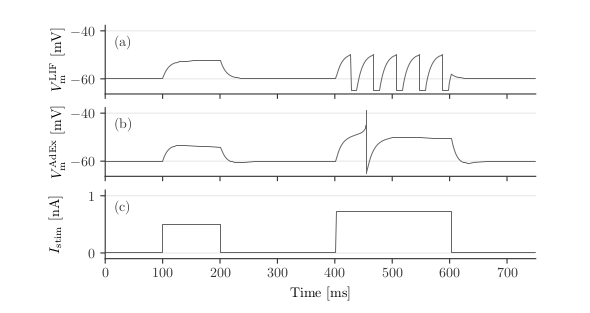
\includegraphics[width=\linewidth]{figures/LIFvsAdEx.png}
	\label{lifvsadex}
	\caption{Difference of membrane dynamics between a \gls{lif} and \gls{adex} neuron, given the same synpatic input. Figure taken from Stradmann, 2019}
\end{figure}

\section{Synaptic Plasticity (Learning)}

Fragen: kapitel zu biological und deep learning einordnen? oder eigenes unterkapitel bestehen lassen?

adapt weights and structure means learning

hebbian what wires together fire s together

LTP (long term potentiation) , STDP (spike timing dependent plasticity) , LTD (long term depression) -> and where are methods like superspike einzuordnen?



\section{Neuromorphic Hardware}

Biologic inspired computing is as popular as it has never been before. IBM started to work on \textit{TrueNorth} in 2008, Intel presented the \textit{Loihi} chip in 2018 and Google started selling the \textit{Coral} dev-board in 2019. Even before neuromorphic hardware caught the attention of the big industry names, several academic projects have already been started. Among others, the EU's Human Brain Project (HBP) funds two promising approaches: \textit{SpiNNaker}, a digital based neuromorphic supercomputer located in Manchester and the \gls{bss}, a mixed-signal accelerated emulation for spiking neural networks based in Heidelberg. The first steps of the latter date back even to the late 80s. (@Billy or Kirchhoff in 1860s).

The \gls{bss2} system, the most recent version of the BrainScaleS platform, is based upon a physical implementation of neurons and synapses. The manufacturing has been outsourced to the Taiwan Semiconductor Manufacturing Company (TSMC) using a standardized $65 \si{nm}$ low-power and low-leakage CMOS technology. The \gls{bss2} successor \gls{bss1} used already a \gls{hicann} chip. Its new revision, the \gls{hx}, contains 512 \gls{adex} neuron circuits, 256 possible synpatic connections per neuron, two plasticity processing units and on-chip routing. The new features have been implemented step by step on smaller prototype systems, e.g. the \gls{dls} where the underlying \gls{lif} neuron model has been tested. To avoid unnecessary costs the size was reduced to $32$ neurons and a corresponding $32 \times 32$ synapse array allows all to all connectivity. Besides the Hagen eXtension, the main features of the \gls{bss2} system are already available on the prototyped versions.  The experiments conducted within this thesis are done either on the \gls{hx} or the \gls{dls}. In the following section the individual parts of the chip are discussed.

%refs: ibm http://www.research.ibm.com/articles/brain-chip.shtml
% coral board:
% Loihi:



\subsection{Architecture of \gls{bss2}}

The design of the \gls{hx} chip can be divided into an analogue and digital core (c.f. figure \ref{HXstructure}). The communication with an external host is streamed out to the controlling Field Programmable Gate Array (FPGA). The existing FPGA solution developed for \gls{bss1} was simply transfered to \gls{bss2}.

\begin{figure}
	\begin{subfigure}[c]{0.5\textwidth}
		\centering
		\caption{}
		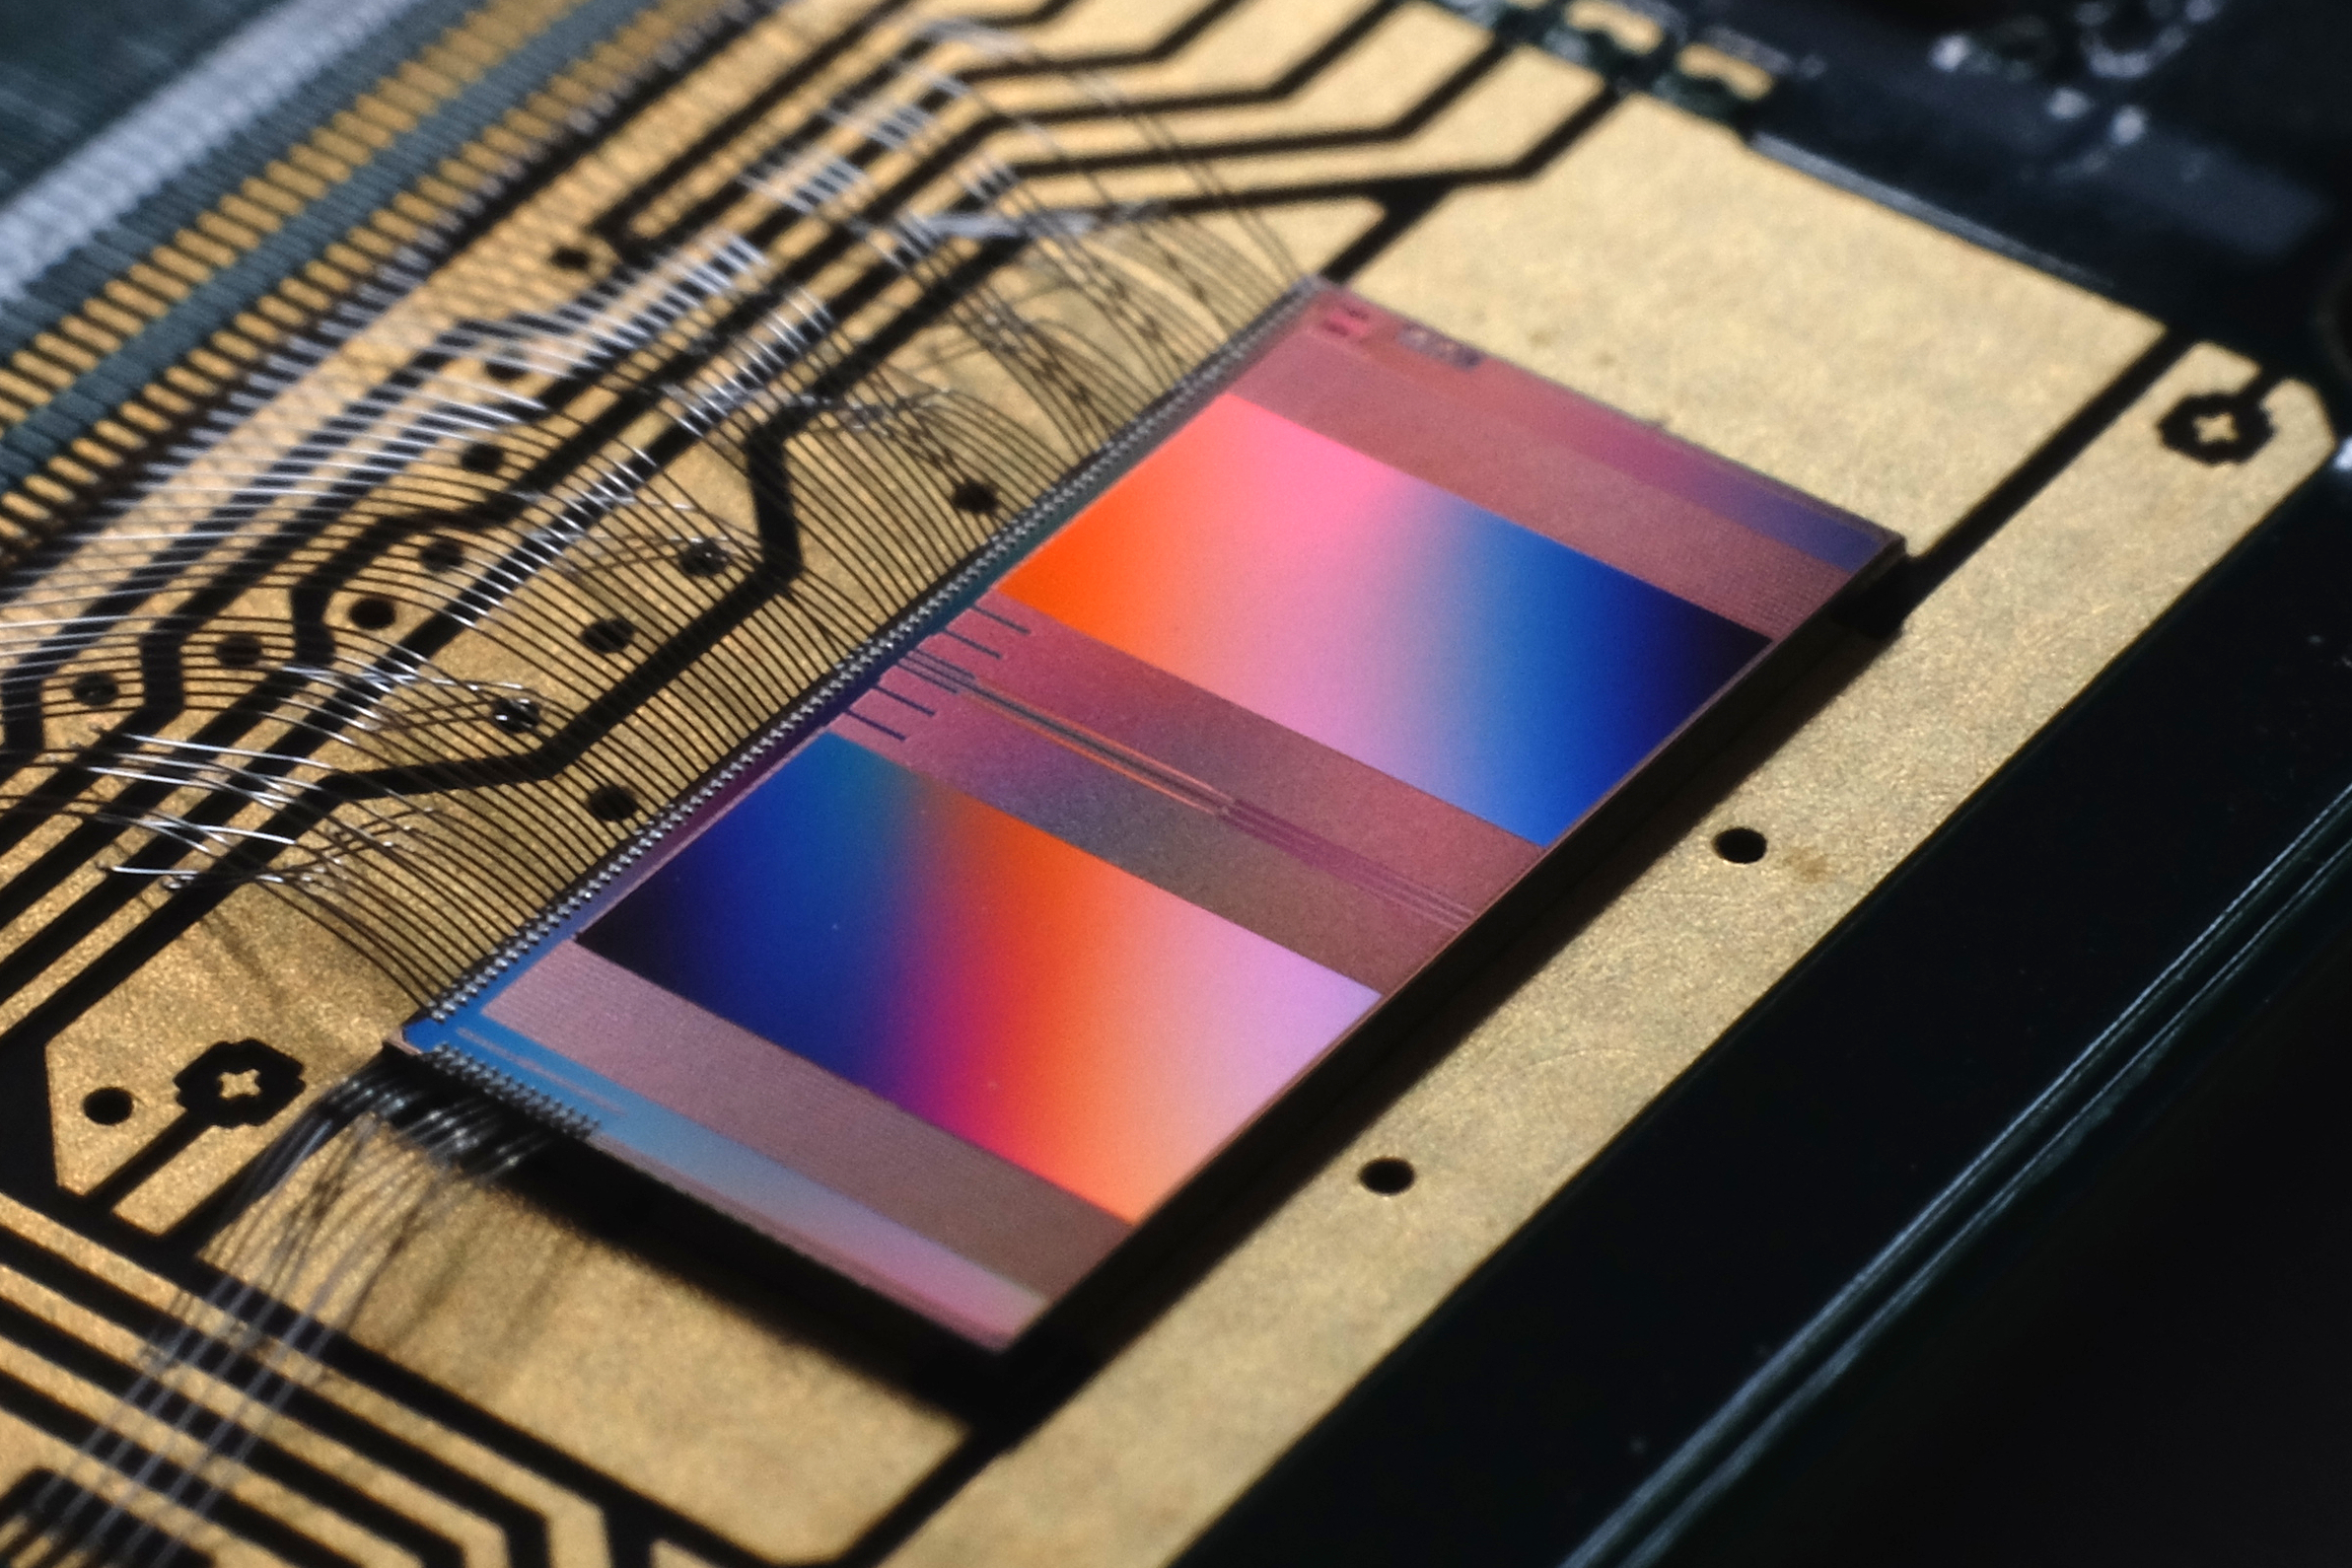
\includegraphics[width=\textwidth]{figures/HXcloseup.JPG}
		\label{hxcloseup}
	\end{subfigure}	
	\begin{subfigure}[c]{0.5\textwidth}
		\centering
		\caption{}
		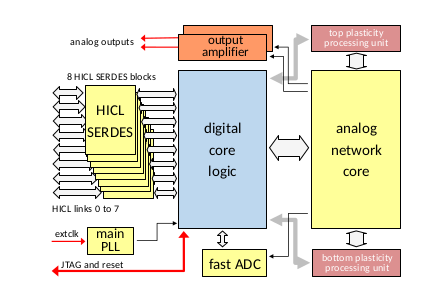
\includegraphics[width=\textwidth]{figures/HXstructure.png}
		\label{hxstructure}
	\end{subfigure}
	\caption{(\subref{hxcloseup}): Close-up of the bonded analog core of the \gls{hx} chip. Picture taken by Müller, 2020. (\subref{hxstructure}): Overview of the architecture of the \gls{hx} chip. Figure taken from \cite{schemmel2017nmda}}
\end{figure}

\subsubsection*{Analogue and Digital Core}
The analogue core implements the neuron dynamics. On the \gls{dls} a current based \gls{lif} neuron model with a total of 32 neurons is used, c.f. \cite{aamir2018dls2neuron}. The dynamics of the chosen \textit{in-silico} implementation of the \gls{lif} neuron has a temporal speed-up factor of 1000 compared to its \textit{in-vivo} counterpart. This acceleration is made possible by the supra-threshold dynamics of CMOS transistors. The biological time constants of neurons and synapses are usually in the order of 10 to 100 milliseconds. The \gls{hx} contains 512 \gls{adex} neurons. An \gls{adex} neuron is basically a more versatile version of the \gls{lif} neuron. The analog model parameters in both chips are tunable by setting bias currents over an 10 bit \gls{dac} \cite{hock13analogmemory}. Each neuron can be controlled and adjusted individually. The 8bit spike counter of the \gls{dls} (one per neuron) has been upgraded to a 10 bit counter in the \gls{hx}. 

The synaptic input is mapped by an $512 \times 256$ synapse array. Each synapse has a 16 bit local \gls{sram} to store weight and information about the presynaptic connections. In addition, two correlation sensors per synapse (causal and anti-causal) record STDP traces and store them in dedicated capacitors. These analog observables can then be processed by a \gls{ppu} via an \gls{adc}. The readout is performed per row and thus a total of 1024 channels (one channel per correlation sensor per synapse) can be accessed by the \gls{cadc}. The \gls{cadc} can also be used to access further observables such as the membrane potential. This feature has not been available on the prototype revisions such as the \gls{dls} and opens up new possibilities for plasticity rules on \gls{hx}.

A highly accelerated analog system requires a fast computation of any plasticity rule. To provide sufficient computational power, the chip is equipped with two \glspl{ppu}, each containing a general-purpose unit that is extended with a special function unit implementing \gls{simd} operations. The special function unit has vector-wise access to the synapse array as well as to the results of the \gls{cadc} and will be further referred to as \textit{vector unit}.

As an additional debugging and observation tool, a \gls{madc} can be accessed from the digital core to readout any available analog observables.

Apart from the spike counters, the digital neuron backend registers any spiking event. Such an event may also come from one of the noise generators or PPUs as well as from an external source. Once a spike has been registered in the digital neuron backend, it is routed back into the synapse array accordingly. 

The link between chip and external host is established via an \gls{fpga} accessing eight serial Low Voltage Differential Signaling (LVDS) links. This interface handles read/write instructions and manages spike event data in both directions. %The FPGA grants access for the PPU to greater memory storages than the one provided on-chip. Access to large training datasets is vital for most learning tasks.